\chapter{\IfLanguageName{dutch}{Stand van zaken}{State of the art}}
\label{ch:stand-van-zaken}
\graphicspath{{../../Images/}} 
% Tip: Begin elk hoofdstuk met een paragraaf inleiding die beschrijft hoe
% dit hoofdstuk past binnen het geheel van de bachelorproef. Geef in het
% bijzonder aan wat de link is met het vorige en volgende hoofdstuk.

% Pas na deze inleidende paragraaf komt de eerste sectiehoofding.

Dit hoofdstuk bevat je literatuurstudie. De inhoud gaat verder op de inleiding, maar zal het onderwerp van de bachelorproef *diepgaand* uitspitten. De bedoeling is dat de lezer na lezing van dit hoofdstuk helemaal op de hoogte is van de huidige stand van zaken (state-of-the-art) in het onderzoeksdomein. Iemand die niet vertrouwd is met het onderwerp, weet nu voldoende om de rest van het verhaal te kunnen volgen, zonder dat die er nog andere informatie moet over opzoeken \autocite{Pollefliet2011}.

Je verwijst bij elke bewering die je doet, vakterm die je introduceert, enz. naar je bronnen. In \LaTeX{} kan dat met het commando \texttt{$\backslash${textcite\{\}}} of \texttt{$\backslash${autocite\{\}}}. Als argument van het commando geef je de ``sleutel'' van een ``record'' in een bibliografische databank in het Bib\LaTeX{}-formaat (een tekstbestand). Als je expliciet naar de auteur verwijst in de zin, gebruik je \texttt{$\backslash${}textcite\{\}}.
Soms wil je de auteur niet expliciet vernoemen, dan gebruik je \texttt{$\backslash${}autocite\{\}}. In de volgende paragraaf een voorbeeld van elk.

\textcite{Knuth1998} schreef een van de standaardwerken over sorteer- en zoekalgoritmen. Experten zijn het erover eens dat cloud computing een interessante opportuniteit vormen, zowel voor gebruikers als voor dienstverleners op vlak van informatietechnologie~\autocite{Creeger2009}.
\newpage
\section{Versiebeheer}
\subsection{Inleiding}
\label{sec:vb_inleiding}
Versiebeheer is een belangrijk concept binnen softwareontwikkeling. Zo waren er in 2018 in het  totaal 100 miljoen projecten op het populaire versiebeheer platform GitHub \autocite{Git2018}. GitHub (sinds 2018 overgenomen door Microsoft) is niet de enige speler op de markt. Er zijn ook nog Code Commit van Amazon en GitLab. Veel bedrijven spelen dus in op de behoefte aan een duidelijk en efficiënt versiebeheersysteem. De vraag stelt zich dan ook: welke behoefte lossen deze systemen op?

Stel volgende scenario voor: Alice en Bob zijn aangenomen om te werken voor bedrijf X. Hun eerste taak is een website ontwikkelen. Ze leggen samen alle vereisten vast, bespreken de verschillende technologieën en gaan aan de slag. Op het einde van de eerste dag hebben ze elk een verschillende pagina gemaakt die ze graag met elkaar delen willen delen. Dit kan door bijvoorbeeld via mail de bestanden door te sturen. Een andere mogelijkheid is de bestanden via fysieke hardware zoals een USB-Stick aan elkaar te geven. Het nadeel is dat de code op twee verschillende plaatsen verspreid zit. Als Bob de code kwijt raakt dan zal deze opnieuw moet worden geschreven. Om dit probleem te voorkomen kan men het project op een centrale server opslaan. Bob en Alice zullen hun veranderingen opslaan op deze centrale server. Zo hebben ze altijd toegang tot elkaars werk. 

Deze manier van werken heeft nadelen. Alice kan per ongeluk een bestand overschrijven of een stuk code verwijderen. Tenzij er back-ups zijn is het originele bestand verloren. Om dit probleem te omzeilen wordt er gebruik gemaakt van het concept van \textbf{versies}. Elke aanpassing die er gemaakt wordt resulteert in een nieuwe versie van het project. Men kan altijd terugkeren naar een eerdere versie. Als Alice dus het stukje code verwijdert in versie 15 kan men terug naar versie 14.

\textcite{Loeliger2009} stelt dat een versiebeheersysteem een middel is om verschillende versies van code te beheren en bij te houden. De auteur onderscheidt volgende drie eigenschappen waaraan dergelijke systemen voldoen:

\begin{itemize}
	\item er wordt gebruik gemaakt van een centraal archief. Binnen dit archief worden alle versies van het project bewaard en bijgewerkt.
	\item het centraal archief geeft toegang tot eerdere versies van het project.
	\item alle veranderingen die worden aangebracht aan het archief worden genoteerd in een centraal logboek.
\end{itemize}

Versiebeheer is geen nieuw concept. Er zijn zoals eerder aangehaald verschillende software oplossingen beschikbaar. Volgens \textcite{Chacon2014} zijn er drie grote categorieën (zie \ref{fig_types_cvs} voor een grafische weergave):

\begin{itemize}
	\item lokale versiebeheersystemen: het centraal archief waar de veranderingen in worden bewaard, staat op een lokale computer. Het grootste voordeel is dat een lokaal systeem zeer makkelijk te onderhouden is en eenvoudig op te stellen. Toch is het niet geschikt om bestanden met elkaar te  delen of samen aan bestanden te werken. Een gekend voorbeeld is RCS (Revision Control System) - zie \ref{sec:RCS} -. \\
	
	\item CVCS: om samen te kunnen werken aan dezelfde bestanden kan een CVCS (Centralised Version Control System) worden gebruikt. In plaats van het archief lokaal bij te houden wordt er gebruik gemaakt van een centrale server. Bestanden worden vervolgens lokaal gekopieerd. Als er veranderingen worden aangebracht zullen deze worden doorgestuurd naar de server.Doordat men verplicht is om de bestanden op een centrale plaats af te halen, kan men deze afschermen. Zo kan men de toegang beperken tot enkel de nodige bestanden per gebruiker. \\
	
Een neveneffect van alles centraal te beheren is het zogenaamde \textit{single point of failure (SPOF)} probleem. Een SPOF is een onderdeel van een systeem dat mocht het uitvallen heel het systeem tot een halt roept. Met andere woorden valt het centraal archief weg heeft niemand nog toegang tot het project. Een mogelijke oplossing voor dit probleem is redundantie. Dit betekent het aanbieden van kopieën. \autocite{Sun2007}\\

	\item DVCS: om het SPOF probleem te voorkomen kan men kopieën maken van het centraal archief. Deze kopieën kunnen vervolgens worden verspreid over verschillende computers. Dit is het uitgangspunt van DVCS (Distributed version control System). Elke gebruiker heeft een lokale kopie van de centrale server. De veranderingen aan de bestanden worden eerst aangebracht in het lokaal archief en vervolgens gesynchroniseerd met de centrale variant.\\

Mocht het centraal aanspreekpunt niet beschikbaar zijn is dit geen probleem. Elke gebruiker heeft immers een volledige back-up van het volledige project. In theorie kan de gebruiker zelfs optreden als nieuwe centrale server.
\end{itemize}


\begin{figure}[h!]
	\centering
	\begin{subfigure}[b]{.5\textwidth}
	\centering
		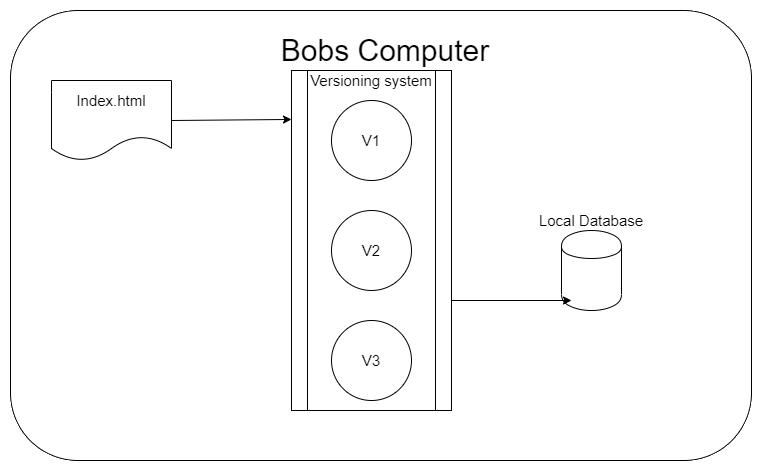
\includegraphics[scale=.3]{LVCS.png}
		\caption[Overzicht structuur Lokale VCS]{Overzicht van de structuur van een Lokale VCS.}
	\end{subfigure}%
	\begin{subfigure}[b]{.5\textwidth}
	\centering
		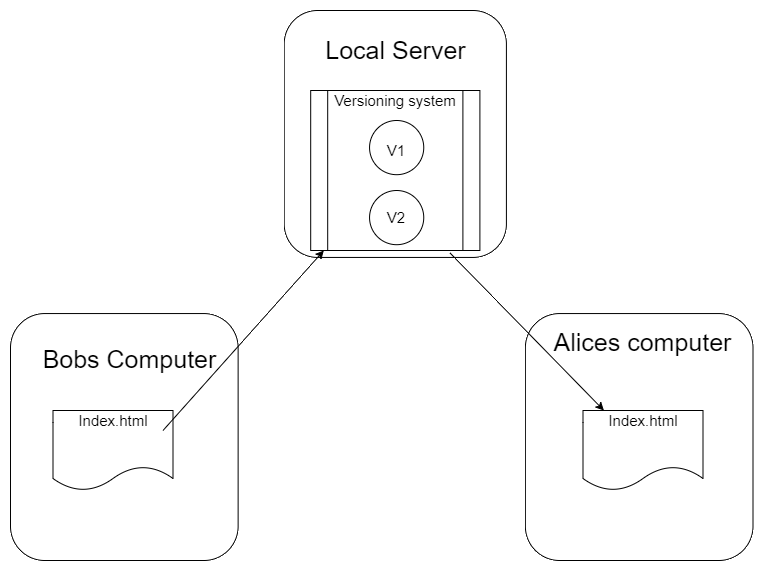
\includegraphics[scale=.3]{CVCS.png}
			\caption[Overzicht structuur CVCS]{Overzicht van de structuur van een CVCS.}
	\end{subfigure}%
	\hfill
	\begin{subfigure}{.5\textwidth}
		\centering
		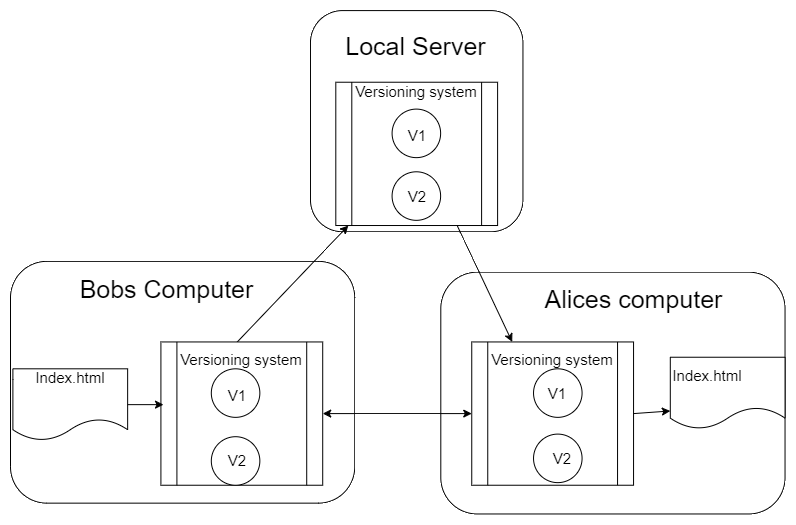
\includegraphics[scale=0.3]{DVCS.png}
	\caption[Overzicht structuur DVCS]{Overzicht van de structuur van een DVCS.}
	\end{subfigure}
	
	\caption[Overzicht types VCS]{Overzicht van de drie types van VCS zoals aangegeven door \textcite{Chacon2014}.}\label{fig_types_cvs}
\end{figure}

	
\subsection{RCS}
\label{sec:RCS}


RCS \textit{(Revision Control System)} is een lokaal versiebeheer systeem. Het wordt voor het eerst beschreven in een artikel geschreven door \textcite{Tichy85rcs}. Het werd verder ontwikkeld binnen het GNU project -Een open source besturingssysteem \footnote{GNU is veel meer dan enkel open source. Het GNU project is sterk verbonden met de ideologie en organisatie van de free software foundation (FSF). Meer informatie omtrent deze organisatie en beweging is te vinden op: \url{https://www.fsf.org/}}- waar het als vervanging voor het CSSC Systeem \autocite{GNUCSSC} werd gebruikt. CSSC is een systeem gebaseerd op SCCS (Source code control system) dat ontworpen is voor UNIX systemen. SCCS is in opdracht van Bell Labs ontwikkeld door \textcite{Rochkind1975}.\\

Voordat RCS op de markt kwam is er nog tal van andere software ontwikkeld. Zo was er CA-Panvalet een gepatenteerde oplossing voor Mainframe computers.\\

Waarom is het interessanter om RCS in detail te bekijken? Veel van de concepten waar het gebruik van maakt zijn aanwezig in moderne systemen (zoals GIT). Het is open source en wordt nog steeds op vrijwillige basis onderhouden, wat aansluit bij de visie van deze bachelorproef.\\

De manier waarop versies worden bijgehouden in RCS -zoals door \textcite{Tichy85rcs} beschreven- is gebaseerd op een boomstructuur -denk aan een stamboom-. Volgens \textcite{Lievens2019}, is een boom een collectie van \textbf{toppen} \textit{(in het Engels ook wel Nodes genoemd)}. Deze toppen hebben een hiërarchische verband.Zo bestaat er bijvoorbeeld een kind-ouder verband. Er zijn twee bijzondere toppen in een boom:

\begin{itemize}
	\item de wortel(\textit{root}): Deze top ligt helemaal aan het begin van de boom. Alle andere toppen zijn afstammelingen van deze top. Het heeft aldus geen ouders.
	\item een blad(\textit{leaf}): Deze top heeft geen kinderen. In tegenstelling tot een wortel kunnen er meerdere bladeren aanwezig zijn.
\end{itemize}

Alle andere toppen worden intermediair genoemd. Elke top heeft mogelijk een aantal kinderen. De diepte van de wortel is nul ($d$=1) en elk kind heeft als diepte: Elk van deze kinderen is op zijn beurt de wortel voor een nieuwe deelboom. Het concept van \textbf{diepte} is belangrijk. 

\begin{equation}
	d_{kind} = d_{ouder} + 1
\end{equation}

%vervang met referentie
Al deze concepten worden ook nog eens grafisch verduidelijkt in de figuur \ref{fig_tree}.

\begin{figure}[h!]
\centering
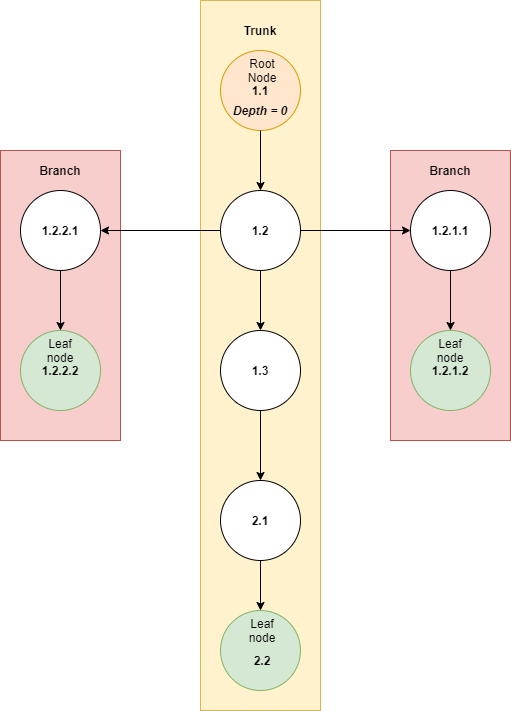
\includegraphics[scale=0.5]{tree1.png}
\caption[Overzicht concepten boomstructuur]{Een overzicht van alle concepten binnen een boomstructuur waar RCS van gebruik maakt.}\label{fig_tree}
\end{figure}

Er kan gebruik gemaakt worden van een boomstructuur om de onderlinge relaties tussen de versies weer te geven. Stel: Bob en Alice zijn bezig aan de hoofdpagina. Bob maakt een initiële versie van de pagina. Vervolgens wilt hij die graag delen met Alice. Hiervoor gebruikt hij het commando om een nieuwe versie aan te maken\footnote{\Verb+ci homepage.html+}. Dit commando wordt \textbf{inchecken} genoemd. Binnen GIT is dit vergelijkbaar met het commando \textit{git push}. Aangezien dit de eerste versie is kan men dit vergelijken met het aanmaken van een wortel. Volgende versies worden kinderen van de vorige versie. Zo wordt versie 1.4 kind van versie 1.3. Inchecken gaat niet alleen onze boomstructuur aanmaken maar ook de extensie \textit{.v} toevoegen (\verb+homepage.html.v+). Het originele bestand wordt ook verwijderd\\

Het bestand krijgt ook een \textbf{versienummer}. Dit versienummer heeft de vorm: $x_1.x_2$.\ $x_1$ (ook wel \textit{release} genoemd) staat voor een grote verandering. Bijvoorbeeld het in productie nemen van een nieuwe versie.$x_2$ (\textit{level}) staat voor een kleinere verandering. Een andere manier om $x_2$ te bekijken is de diepte met als wortel de laatste release ($x_1$). 1.1 is het versienummer van de wortel die Bob heeft aangemaakt. 1.4 is het derde kind van de wortel.Elke check-in zal het level ($x_2$) met één verhogen. Het release nummer ($x_1$) wordt manueel verhoogd door middel van de \textit{-r} optie bij check-in \footnote{\Verb+ci -r2 homepage.html+}. Bij branches is er ook nog spraken van $x_3$ en $x_4$ zie \ref{par:branches}.\\

Deze manier van versies te bestempelen wordt nog steeds gebruikt. Het is echter niet de enige manier. \textit{Semantic versioning} is een gekend alternatief. Het concept van versienummers bestaat in Git onder de vorm van \textit{tags} (\ref{sec:GIT}).\\

Er is nu een bestand onder de vorm \verb+homepage.html.v+. Hoe kan Alice nu dit bestand aanpassen en een nieuwe versie publiceren? Alice zal het bestand moeten \textbf{uitchecken}.Dit kan ze doen door middel van het commando \verb+co+ en de naam van het bestand \footnote{(\Verb+co homepage.html+)} . Het uitchecken is aldus het verkrijgen van een specifieke versie uit het archief. Als er geen specifieke versie wordt meegegeven wordt de laatste versie opgehaald. Om een specifieke versie op te halen kan er gebruik gemaakt worden van de optie -r  \footnote{(\Verb+co -r1.1 homepage.html+)} . Alice heeft nu een kopie van het originele bestand gekregen. Merk op dat in tegenstelling tot inchecken ons archief niet wordt verwijderd. Vervolgens kan ze in deze lokale kopie wijzigingen aanbrengen. Tot slot wordt het bestand weer aan het lokaal archief toegevoegd door middel van inchecken. Het equivalent van \verb+co+ binnen git is \verb+git pull+.\\

\begin{wrapfigure}{r}{0.5\textwidth}
\begin{center}
  	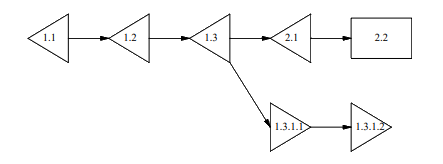
\includegraphics[scale=0.6]{deltas.png}
\end{center}
\caption[Voorbeeld van deltas.]{Een voorbeeld van deltas.De Trunk bevat een series van achterwaardse deltas terwijl alle branches enkel voorwaardse deltas bevatten. Grafiek afkomstig uit \textcite{Tichy85rcs}}\label{fig_deltas}
\end{wrapfigure}

Hoe worden de verschillen tussen de versies bijgehouden in ons lokaal archief? Een mogelijke oplossing zou zijn om alle versies van het bestand afzonderlijk bij te houden. Dit vraagt veel opslagruimte. RCS gebruikt voor dit probleem het concept van \textbf{deltas}. Een delta houdt bij welke regels veranderd zijn ten opzichte van de vorige versie. Doordat de delta enkel de relevante lijnen bijhoudt wordt de opslag beperkt \footnote{De delta wordt opgebouwd aan de hand van het GNU commando diff \url{https://www.gnu.org/software/diffutils/}}. Er zijn twee types van deltas: \textbf{voorwaardse deltas} en \textbf{achterwaardse deltas}. Bij het inchecken van een nieuwe versie zal de vorige versie worden vervangen door een achterwaardse delta. Zit men momenteel op versie 1.3 en  vraagt men versie 1.2 dan zal de achterwaardse delta van versie 1.2 worden toegepast op versie 1.3. (Voorwaardse deltas komen aan bod in het gedeelte over branching (\ref{par:branches}). Het concept van deltas wordt nog eens verduidelijkt door een voorbeeld in de appendix -zie \ref{ch:voorbeeld-rcs}-.)\\

Inchecken en uitchecken ligt aan de basis van het archiefsysteem. Toch is er nog een probleem aanwezig met deze manier van werken. Stel dat Alice en Bob gelijktijdig wijzigingen aanbrengen aan een bestand. Ze willen dit bestand elk afzonderlijk publiceren.  Hierdoor ontstaan er twee versies die afstammen van één gezamenlijke versie. De boomstructuur wordt in twee gesplitst. Dit is niet mogelijk aangezien een versie altijd uniek moet zijn. Hoe kan men verzekeren dat elke versie slechts één kind heeft (op dezelfde branch)? Dit probleem wordt opgelost door \textbf{sloten}(engels=lock).Dit concept geeft gebruikers de mogelijkheid om een versie te  versleutelen. Terwijl een versie versleuteld is kan niemand anders wijzigingen aanbrengen. Andere gebruikers kunnen deze nog bekijken. Op het moment dat Bob zijn versie gaat uitchecken kan hij deze versleutelen (door middel van de \textit{-l} optie bij het co commando). Hierdoor kan Alice geen nieuwe versie meer aanmaken tot Bob zijn wijzigingen heeft doorgevoerd. Met andere woorden zolang Bob het slot niet vrijgeeft kunnen er geen nieuwe versies worden aangemaakt\footnote{In sommige gevallen kan het slot ook worden 'geforceerd' mocht Bob bijvoorbeeld ziek vallen}. Deze manier van werken heeft een zichtbaar nadeel. Alice is verplicht om te wachten op Bobs nieuwe versie alvorens ze veranderingen kan aanbrengen. Git gebruikt het concept van sloten niet. Daar maakt men gebruik van \textbf{merges} om dit zelfde probleem aan te pakken %\ref{sec:GIT}%.

\subsubsection{Opmerkingen}
In het originele artikel wordt de klemtoon gelegd op het onderling delen van de verschillende versies. Hierdoor kan men de indruk krijgen dat er een centrale server betrokken is. Dit is niet het geval. De software is ontworpen om op één besturingssysteem uitgevoerd te worden. Volgens \textcite{Debian2020} is GNU aangezien het gebaseerd is op UNIX een \textit{multi-user os}. Dat wil zeggen dat meerdere gebruikers het systeem tezelfdertijd kunnen gebruiken door middel van een terminal connectie. Hierdoor kan men onderling de bestanden delen ondanks dat men niet gaat werken in een CVCS.

\subsection{branches}
\label{par:branches}
\subsubsection{Duiding}
Door het principe van sloten en inchecken lijkt het alsof elke versie exact één opvolger heeft. Zo zal versie 1.3 de opvolger zijn van 1.2. Toch kunnen er zoals in een stamboom zich vertakkingen voordoen. De vertakkingen worden \textbf{Branches} genoemd. De hoofdboom (niet vertakte toppen die afstammen van de wortel) wordt de \textbf{trunk} genoemd. Dit principe kan men het best demonstreren aan de hand van een figuur. Zo kan men zien in figuur \ref{fig_tree} dat er twee vertakkingen zijn op versie 1.2. Het principe van vertakkingen lijkt op eerste zich complex en onoverzichtelijk. \textcite{Tichy85rcs} geeft enkele redenen om dit toch toe te passen.

\begin{enumerate}
\item Doorvoeren van veranderingen in oude versies: Stel dat een bedrijf gebruikt een oude versie van een software product ontwikkeld met behulp van RCS. Ze ontdekken een fout in deze oude versie en vragen een oplossing. Aangezien er in de tussentijd nieuwere versies zijn is dit niet evident. Het bedrijf zou volledig moeten overstappen op de nieuwste versie alvorens een aanpassing kan gebeuren. Om deze situatie te vermijden kan men gebruik maken van vertakkingen. Zo kan men een vertakking maken op de gewenste versie en kleine aanpassingen doorvoeren.\\
\item Andere implementaties: Stel dat een ontwikkelaar een nieuwe stuk code wilt uittesten. Deze heeft niet het gewenste resultaat. Mocht dit stuk code bewaard worden op de hoofdboom (\textit{trunk}) dan is er een onstabiele versie gepubliceerd. Een gebruiker die op dat moment de recentste versie opvraagt krijgt dus een niet werkend product.\\
Door branches te gebruiken kan men ervoor zorgen dat er enkel werkend versie op de hoofdboom terecht komen. Nieuwe stukken code worden eerst geïsoleerd en getest alvorens opgenomen te worden. Op die manier blijft het archief in een overzichtelijke en stabiele vorm.
\end{enumerate}

\begin{wrapfigure}{L}{0.5\textwidth}
\begin{center}
  	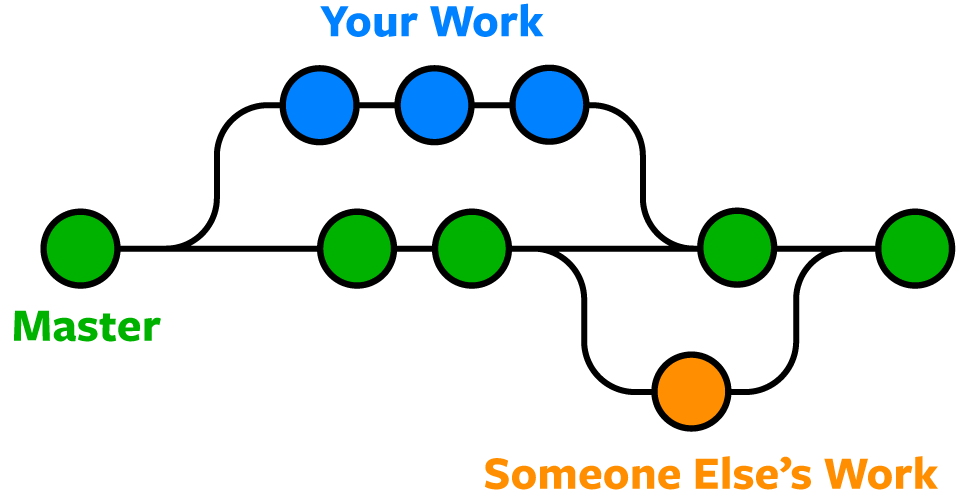
\includegraphics[scale=0.2]{git-branches-merge.png}
\end{center}
\caption[Voorbeeld merge proces.]{Een voorbeeld van een merge proces. Eerst wordt er een branch aangemaakt die na drie versies terug in de master wordt gemerged. Grafiek gepubliceerd door \textcite{NobleDesktop2018}}\label{fig_merge}
\end{wrapfigure}

Door middel van vertakkingen kan code worden geschreven en de hoofdboom stabiel gehouden. Hierdoor is het een elegante manier om samen te werken binnen grote teams en projecten. Eenmaal de code klaar is voor productie kan men deze gaan publiceren op de hoofdboom. Dit concept noemen we \textbf{mergen}. Dit principe wordt geïllustreerd door de figuur \ref{fig_merge}.

%todo uitleg van RCS branching en forward deltas

\subsubsection{Flows}
Er is echter nog een grote vraag die niet beantwoord is: wanneer moet men gaan vertakken?

De eerste reden aangehaald door \textcite{Tichy85rcs} -het doorvoeren van veranderingen- is minder relevant binnen de context van DVCS. Er wordt namelijk niet meer op een gezamenlijk archief gewerkt maar op een lokale kopie. Het bedrijf kan dus op hun eigen kopie lokaal veranderingen aanbrengen .De tweede reden is echter wel belangrijk. Stel een project met honderden bestanden en verschillende ontwikkelaars. In zo een omgeving kunnen veranderingen soms onvoorspelbare gevolgen hebben. Ontwikkelaars kunnen het project vertakken, wijzigen en testen alvorens men het in productie neemt. Dit is het principe achter \textbf{feature branches}.\\

%Voeg meer bron vermeldingen toe
Er zijn echter een aantal verschillende werkwijzen om branching te gaan gebruiken. Een mogelijke werkwijze is dat vermeld in het artikel van \textcite{Bird2012}. Het artikel benadrukt het belang van \textit{levende} takken. Bij grote software projecten loopt men het risico dat er veel aftakkingen worden gemaakt die niet worden gebruikt (\textbf{branchmania}).

\begin{figure}
\begin{center}
  	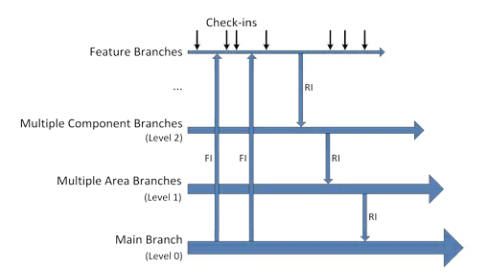
\includegraphics[scale=1]{microsoft-branching.png}
\end{center}
\caption[Voorbeeld flow]{Flow zoals vermeld in het artikel van  \textcite{Bird2012}}\label{fig_mic_flow}
\end{figure}

De werkwijze die wordt geïllustreerd in figuur \ref{fig_mic_flow} probeert om het aantal vertakkingen zo klein mogelijk te houden. Elke ontwikkelaar gaat zijn code schrijven op een feature branch. Het risico hiervan is dat men op den duur niet meer compatibel wordt met de hoofdbom. Er kunnen sinds de vertakking immers verschillende andere versies gepubliceerd zijn. Daarom wordt gewerkt met twee tussen branches. Hier test men of de code compatibel is met de verschillende andere onderdelen van de software. Het proces waarbij men feature branches gaat integreren in andere tussen branches noemt men ook wel \textbf{Reverse integration} -aangeduid als RI op de figuur-. Een ander principe dat gebruikt wordt is dat van \textbf{Forward integration}. Hierbij worden de nieuwe versies van de hoofdbranch (ook wel master genoemd) geplaatst op de feature branch. Zo blijft de feature branch compatibel met alle veranderingen.

%toevoegen van GIT Flow
%toevoegen van Trunk based developmet
Buiten de methodiek voorgesteld door \textcite{Bird2020} bestaat er ook GIT Flow en Trunk based development. 


%\subsection{GIT}
%\label{sec:GIT}

\subsection{Conclusie}
De verschillende types van versiebeheer systemen -zoals besproken in \ref{sec:vb_inleiding}- hebben een gemeenschappelijke eigenschap. De bestanden en in veel gevallen het archief staat integraal opgeslagen op computers. Bij lokale versiebeheersystemen en CVCS staat het zelfs op één centrale computer. Dit introduceert het probleem van een SPOF (Single point of failure).DVCS vermeid dit probleem door gebruikers kopieën te geven van het archief. Valt de centrale computer weg dan heeft elke gebruiker een back-up. Veranderingen tussen lokale versies en die op de centrale computer moet manueel gesynchroniseerd worden. Hierdoor heeft men in grote mate controle over wat er centraal wordt opgenomen. Het nadeel is dat er veel lokale kopieën zijn en veranderingen niet altijd worden gesynchroniseerd. Op deze manier heeft niet iedereen toegang tot de laatste veranderingen. Het zou dus een verbetering zijn mocht er een systeem bestaan dat één centraal archief ondersteund zonder SPOF. Dit lijkt op eerste zicht niet mogelijk, aangezien er één centraal aanspreekpunt moet zijn. Toch is dit probleem al eerder opgelost onder de vorm van peer-to-peer (afgekort tot p2p) netwerken.\\

P2P is voornamelijk bekend onder de vorm van file-sharing netwerken zoals Napster. \textcite{Chawathe2003} stellen dat Napster één van de eerste systemen was die erin slaagde om een succesvol netwerk uit te bouwen. Bij dit netwerk worden files niet opgevraagd aan een centrale server. In plaats hiervan gebruikt men een netwerk van \textbf{peers} -zie \ref{ch:p2p}-. Door de principes van dit type van netwerken toe te passen kan men een centraal archief op een gedistribueerde manier opslaan. Zo behoud men het voordeel van CVCS zonder een SPOF. \\

De doelstellingen van deze bachelorproef is om een werkend P2P versiebeheer systeem te gaan implementeren. Hiervoor moet men afbakenen welke functionaliteiten deze implementatie moet voorzien. In vorige paragrafen werden de verschillende concepten besproken. Hieronder volgt een oplijsting van deze verschillende concepten alsook een korte uitleg. Hierbij worden de terminologie en concepten van Git gebruikt. Deze worden vervolgens meegenomen naar volgende hoofdstukken, waar een implementatie wordt voorzien.

\begin{table}[h!]
	\centering
	\begin{tabular}{ |p{2cm}|p{12cm}|}
 		\hline
 		\multicolumn{2}{|c|}{\large \textbf{Concepten binnen versiebeheer}} \\
 		\hline
 		\textbf{Begrip}	& \textbf{Uitleg}\\
 		\hline
 		\textbf{Archief} & Een centrale plaats voor het bijhouden van bestanden. De wijzigingen van deze gearchiveerde bestanden worden bijgehouden. Men kan zowel historische als recente versies van het bestand opvragen. Alsook van het gehele archief.\\
 		\hline
 		\textbf{Versies} & Elke wijziging binnen het archief leid tot een nieuwe versie. Men kan de verschillende versies ten alle tijden raadplegen. Men kan ook oudere versies gaan gebruiken voor branching. In extreme gevallen kan een archief volledig worden terug gedraaid naar een eerdere versie.\\
 		\hline
		\textbf{Logboek} & Een bestand waar alle wijzigingen worden bijgehouden. Het logboek is ook onderdeel van het archief. \\
		\hline
		Pushing	& Het principe waarbij we wijzigingen die we lokaal aanbrengen gaan synchroniseren met de centrale server.\\
		\hline
		Pulling & Het binnenhalen van veranderingen aangebracht op het centraal archief naar een lokale kopie.\\
		\hline
		Clonen & Het aanmaken van een lokale kopie van een centraal archief. \\
		Branching & Het voorzien van alternatieve vertakkingen van het archief. \\
		\hline
	\end{tabular}
	\label{tbl_concepts}
	\caption{Concepten binnen versiebeheer systemen.}
\end{table}
\section{Peer-to-peer en IPFS}
\label{ch:p2p}